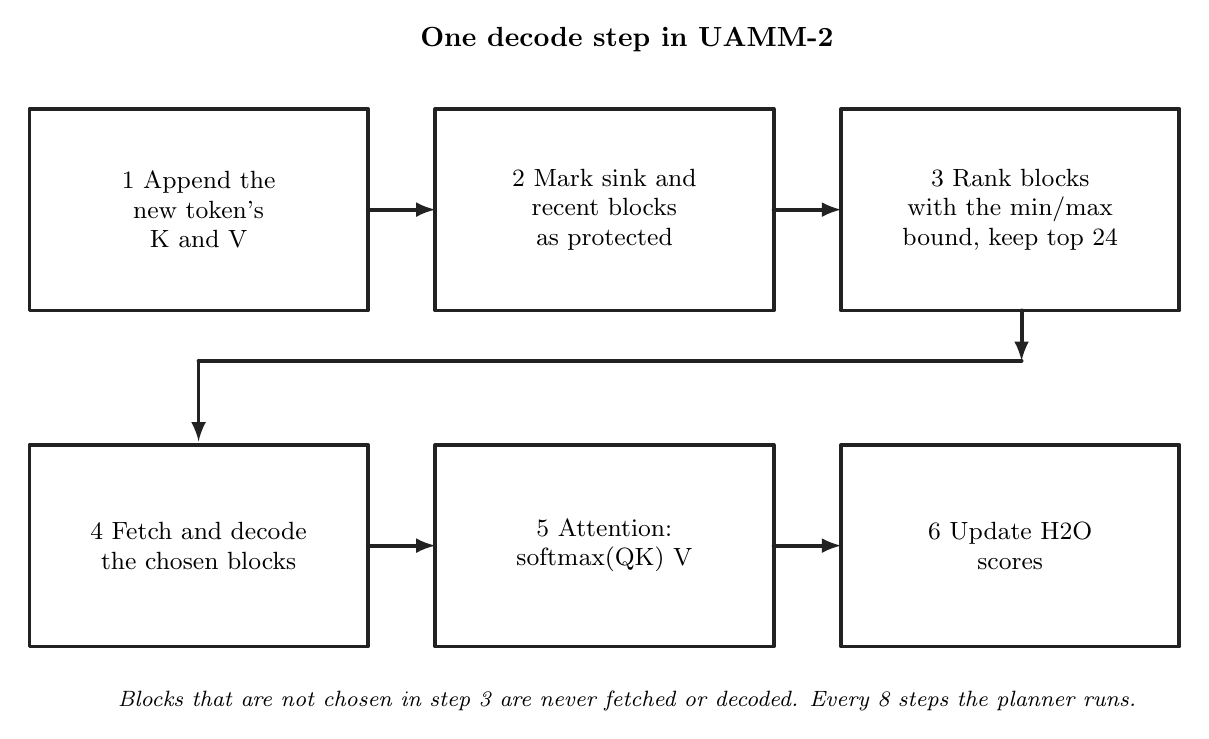
\begin{tikzpicture}[line cap=round,line join=round]
\draw[line width=1.38pt,draw={rgb,255:red,34;green,34;blue,34},fill={rgb,255:red,255;green,255;blue,255}] (0.113in,2.128in) rectangle (1.804in,3.136in);
\draw[line width=1.38pt,draw={rgb,255:red,34;green,34;blue,34},fill={rgb,255:red,255;green,255;blue,255}] (2.142in,2.128in) rectangle (3.833in,3.136in);
\draw[line width=1.38pt,draw={rgb,255:red,34;green,34;blue,34},fill={rgb,255:red,255;green,255;blue,255}] (4.171in,2.128in) rectangle (5.862in,3.136in);
\draw[line width=1.38pt,draw={rgb,255:red,34;green,34;blue,34},fill={rgb,255:red,255;green,255;blue,255}] (0.113in,0.448in) rectangle (1.804in,1.456in);
\draw[line width=1.38pt,draw={rgb,255:red,34;green,34;blue,34},fill={rgb,255:red,255;green,255;blue,255}] (2.142in,0.448in) rectangle (3.833in,1.456in);
\draw[line width=1.38pt,draw={rgb,255:red,34;green,34;blue,34},fill={rgb,255:red,255;green,255;blue,255}] (4.171in,0.448in) rectangle (5.862in,1.456in);
\draw[line width=1.38pt,draw={rgb,255:red,34;green,34;blue,34}] (5.073in,1.876in) -- (0.958in,1.876in);
\node[align=center,text={rgb,255:red,0;green,0;blue,0},font=\fontsize{9.1pt}{10.7pt}\selectfont,inner sep=0pt] at (0.958in,2.632in) {1  Append the \\ new token's \\ K and V};
\draw[-latex,line width=1.38pt,draw={rgb,255:red,34;green,34;blue,34}] (1.804in,2.632in) -- (2.142in,2.632in);
\node[align=center,text={rgb,255:red,0;green,0;blue,0},font=\fontsize{9.1pt}{10.7pt}\selectfont,inner sep=0pt] at (2.987in,2.632in) {2  Mark sink and \\ recent blocks \\ as protected};
\draw[-latex,line width=1.38pt,draw={rgb,255:red,34;green,34;blue,34}] (3.833in,2.632in) -- (4.171in,2.632in);
\node[align=center,text={rgb,255:red,0;green,0;blue,0},font=\fontsize{9.1pt}{10.7pt}\selectfont,inner sep=0pt] at (5.016in,2.632in) {3  Rank blocks \\ with the min/max \\ bound, keep top 24};
\node[align=center,text={rgb,255:red,0;green,0;blue,0},font=\fontsize{9.1pt}{10.7pt}\selectfont,inner sep=0pt] at (0.958in,0.952in) {4  Fetch and decode \\ the chosen blocks};
\draw[-latex,line width=1.38pt,draw={rgb,255:red,34;green,34;blue,34}] (1.804in,0.952in) -- (2.142in,0.952in);
\node[align=center,text={rgb,255:red,0;green,0;blue,0},font=\fontsize{9.1pt}{10.7pt}\selectfont,inner sep=0pt] at (2.987in,0.952in) {5  Attention: \\ softmax(QK) V};
\draw[-latex,line width=1.38pt,draw={rgb,255:red,34;green,34;blue,34}] (3.833in,0.952in) -- (4.171in,0.952in);
\node[align=center,text={rgb,255:red,0;green,0;blue,0},font=\fontsize{9.1pt}{10.7pt}\selectfont,inner sep=0pt] at (5.016in,0.952in) {6  Update H2O \\ scores};
\draw[-latex,line width=1.38pt,draw={rgb,255:red,34;green,34;blue,34}] (5.073in,2.128in) -- (5.073in,1.876in);
\draw[-latex,line width=1.38pt,draw={rgb,255:red,34;green,34;blue,34}] (0.958in,1.876in) -- (0.958in,1.473in);
\node[anchor=south,align=center,text={rgb,255:red,0;green,0;blue,0},font=\fontsize{10.2pt}{12.0pt}\selectfont\bfseries,inner sep=0pt] at (3.100in,3.416in) {One decode step in UAMM-2};
\node[anchor=south,align=center,text={rgb,255:red,0;green,0;blue,0},font=\fontsize{8.0pt}{9.4pt}\selectfont\itshape,inner sep=0pt] at (3.100in,0.123in) {Blocks that are not chosen in step 3 are never fetched or decoded. Every 8 steps the planner runs.};
\end{tikzpicture}
